\subsection{Variation 1.1}
\textbf{Question:} Which of the following statements about race conditions are correct? Please select the two correct answers.

\textbf{Correct Answer(s):}
\begin{itemize}
    \item Race conditions occur when multiple processes access shared resources without proper synchronization. 
    \item The outcome of a race condition depends on the order of execution of processes. 
\end{itemize}

\textbf{Incorrect Answers:}
\begin{itemize}
    \item Race conditions can be avoided by allowing processes to update shared data simultaneously. 
    \item Race conditions are harmless and do not affect program behavior. 
    \item Locks or synchronization mechanisms completely prevent race conditions. 
\end{itemize}

\textbf{Solution \& Feedback:}
\begin{itemize}
    \item Race conditions can be avoided by allowing processes to update shared data simultaneously.\\
    Incorrect, as simultaneous updates without proper synchronization cause race conditions, rather than avoiding them. 
    \item Race conditions are harmless and do not affect program behavior. \\
    Incorrect, because race conditions can lead to unexpected and incorrect program behavior, which can be hard to debug. 
    \item Locks or synchronization mechanisms completely prevent race conditions. \\
    Incorrect because improper or incomplete use of locks or synchronization mechanisms can still lead to race conditions. 
\end{itemize}
\subsection{Variation 1.2}
\textbf{Question:} Which of the following statements about race conditions are correct? Please select the two correct answers. \\
\textbf{Correct Answer}
\begin{itemize}
    \item Race conditions arise when multiple processes read and write shared data. 
    \item Race conditions can occur due to context switches at arbitrary times. 
\end{itemize}
\textbf{Solution \& Feedback:}
\begin{itemize}
    \item The order of execution in race conditions is predictable and consistent. [cite: 138] Incorrect, as the execution order in race conditions is often unpredictable. [cite: 139]
    \item Processes operating with outdated information contribute to race conditions. [cite: 140] Incorrect, as the outdated information is a consequence of the race conditions, not the cause. [cite: 140]
    \item Using multiple threads eliminates the possibility of race conditions. [cite: 141] Incorrect, as multiple threads often introduce race conditions if not synchronized properly. [cite: 141]
\end{itemize}

\subsection{Variation 1.3}
\textbf{Question} Which of the following statements about race conditions are correct? Please select the two correct answers. \\
\textbf{Correct Answer}
\begin{itemize} 
    \item Shared data may become inconsistent. 
    \item The final value of shared data depends on the order of execution.
\end{itemize}
\textbf{Solution \& Feedback:}
\begin{itemize}
    \item Race conditions simplify the debugging process for concurrent systems. [cite: 142] Incorrect, as debugging becomes harder due to non-deterministic and unpredictable behavior. [cite: 142]
    \item Processes involved in a race condition always produce the same results. [cite: 142] Incorrect, as the results are often different depending on execution order. [cite: 142]
    \item Using multiple threads eliminates the possibility of race conditions. [cite: 142] Incorrect, as multiple threads often introduce race conditions if not synchronized properly. [cite: 142]
\end{itemize}

\subsection{Variation 2.1}
\textbf{Question} Socket addresses are made up of IP addresses and another identifier. The purpose of the other identifier is to uniquely identify... \\
\begin{tabularx}{\textwidth}{|X|X|}
    \hline
    \textbf{Correct Answer(s)} & \textbf{Incorrect Answers} \\
    \hline
    ...a particular application process running on a given host machine on the network. [cite: 143] & ...a particular host machine on the network. [cite: 143] \\
        & ...a host machine running a given application on the network. [cite: 143] \\
        & ...a particular application process, and the host machine running it, on the network. [cite: 143] \\
    \hline
\end{tabularx}
\subsection{Variation 2.2}
\textbf{Question} Socket addresses are made up of port numbers and another identifier. The purpose of the other identifier is to uniquely identify... \\
\begin{tabularx}{\textwidth}{|X|X|}
    \hline
    \textbf{Correct Answer(s)} & \textbf{Incorrect Answers} \\
    \hline
    ...a particular host machine on the network. [cite: 144] & ...a particular application process running on a given host machine on the network. [cite: 144] \\
        & ...a host machine and a given user on the network. [cite: 144] \\
        & ...a particular application process, and the host machine running it, on the network. [cite: 144] \\
    \hline
\end{tabularx}
\subsection{Variation 2.3}
\textbf{Question} Socket addresses are made up of two identifiers. The purpose of this combination is to uniquely identify... \\
\begin{tabularx}{\textwidth}{|X|X|}
    \hline
    \textbf{Correct Answer(s)} & \textbf{Incorrect Answers} \\
    \hline
    ...a particular application process, and the host machine running it, on the network. & ...a particular host machine on the network. \\
        & ...a particular application process on the network. \\
        & ...a particular host machine and a user on the network. \\
    \hline
\end{tabularx}

\textbf{Solution \& Feedback:}
{\color{red}
Socket address are made up of IP addresses (which uniquely identify a particular host machine on the network) and port numbers (which uniquely identify a particular application process running on a given host machine on the network). When combined, they uniquely identify a particular application process, and the host machine running it, on the network. 
}
\subsection{Variation 3.1}
\textbf{Question} A host machine is communicating with an HTTP/1.1 server. Tick the two correct statements about the Transport Layer protocol used in this communication session. \\
\begin{tabularx}{\textwidth}{|X|X|}
    \hline
    \textbf{Correct Answer(s)} & \textbf{Incorrect Answers} \\
    \hline
    The protocol establishes a logical connection between the host and the server. & The protocol is a best-effort service. \\
    The protocol provides flow and congestion controls. & The protocol's header is 8 bytes. \\
    \hline
\end{tabularx}

\subsection{Variation 3.2}
\textbf{Question} A host machine is communicating with an SMTP mail server. Tick the two correct statements about the Transport Layer protocol used in this communication session. \\
\begin{tabularx}{\textwidth}{|X|X|}
    \hline
    \textbf{Correct Answer(s)} & \textbf{Incorrect Answers} \\
    \hline
    The protocol utilises sequence and acknowledgement numbers. & The protocol is connectionless. \\
    The protocol provides flow and congestion controls. & The protocol's header is 8 bytes. \\
    \hline
\end{tabularx}

\subsection{Variation 3.3}
\textbf{Question} A host machine is communicating with a DNS server. Tick the two correct statements about the Transport Layer protocol used in this communication session. \\
\begin{tabularx}{\textwidth}{|X|X|}
    \hline
    \textbf{Correct Answer(s)} & \textbf{Incorrect Answers} \\
    \hline
    The protocol is connectionless. & The protocol utilises sequence and acknowledgement numbers. \\
    The protocol's header is 8 bytes. & The protocol establishes a logical connection between the host and the server. \\
    \hline
\end{tabularx}

\textbf{Solution \& Feedback:}
{\color{red}
HTTP/1.1 and SMPT use the TCP Transport Layer protocol. TCP in a connection-oriented protocol which provides a variety of transport services, such as flow and congestion controls and the utilizations of sequence and acknowledgement numbers to support reliable data transfer. 
Meanwhile, DNS uses UDP, which is a best-effort, connectionless Transport Layer protocol which has fewer transport services and, thus, a more lightweight header (only 8 bytes). \\
}
\subsection{\textcolor{red}{Variation 4.1}}

\textbf{Question} Suppose Host A wants to send a large file to Host B. The path from Host A to Host B has four links of rates \(R1=700\) Kbps, \(R2=3\) Mbps, \(R3=500\) Kbps and \(R4=2\) Mbps. Assuming no other traffic in the network, approximately, how long will it take (in seconds) to transfer a file of 1400 MiB from Host A to Host B? \\
Please note:
1 \(1~MiB=1024~KiB\), and 1 \(KiB=1024\) bytes (for file sizes)
\(1~Mbps=1,000\) Kbps and \(1~Kbps=1,000~bits/sec\) (for network) \\
\begin{tabular}{|c|c|}
    \hline
    \textbf{Correct Answer(s)} & \textbf{Incorrect Answers} \\
    \hline
    23488.10 sec & 2936.01 sec \\
        & 3914.68 sec \\
        & 489.33 sec \\
    \hline
\end{tabular}
\textbf{Solution \& Feedback:}
Effective throughput on this network will be 500 Kbps (the lowest rate).
File size (in KiB) \(=1400 \times 1024 = 1433600\) KiB \\
File size (in Bytes) \(=1433600 \times 1024 = 1468006400\) Bytes\\
File size (in Bits) = \(1468006400 \times 8 = 11744051200\) Bits\\
File transfer time will be \(=11744051200/(500 \times 1000)=23488.10\) seconds.\\

\subsubsection{Variation 4.2}

\textbf{Question} Suppose Host A wants to send a large file to Host B. The path from Host A to Host B has four links of rates \(R1=800\) Kbps, \(R2=600\) Kbps, \(R3=3\) Mbps and \(R4=5~Mbps\). Assuming no other traffic in the network, approximately, how long will it take (in seconds) to transfer a file of 1500 MiB from Host A to Host B?\\
Please note:\\
1 \(MiB=1024~KiB\) and 1 \(KiB=1024\) bytes (for file sizes)
1 \(Mbps=1,000\) Kbps and \(1~Kbps=1,000~bits/sec(\) for network) \\
\begin{tabular}{|c|c|}
    \hline
    \textbf{Correct Answer(s)} & \textbf{Incorrect Answers} \\
    \hline
    20971.52 sec & 2621.44 sec  \\
        & 2516.58 sec  \\
        & 314.57 sec  \\
    \hline
\end{tabular}

\textbf{Solution \& Feedback:}\\
Effective throughput on this network will be 600 Kbps (the lowest rate). \\
File size (in KiB) \(=1500 \times 1024=1536000\) KiB  \\
File size (in Bytes) \(=1536000 \times 1024=1572864000\) Bytes \\
File size (in Bits) = \(1572864000 \times 8=12582912000\) Bits \\
File transfer time will be \(=12582912000/(600 \times 1000)=20971.52\) seconds. \\

\subsection{Variation 4.3}
\textbf{Question} Suppose Host A wants to send a large file to Host B. The path from Host A to Host B has four links of rates \(R1=900\) Kbps, \(R2=800\) Kbps, \(R3=3\) Mbps and \(R4=700\) Kbps. Assuming no other traffic in the network, approximately, how long will it take (in seconds) to transfer a file of 1700 MiB from Host A to Host B?\\
Please note:\\
1 \(MiB=1024~KiB\), and 1 \(KiB=1024\) bytes (for file sizes)
\(1~Mbps=1,000\) Kbps and \(1~Kbps=1,000~bits/sec\) (for network) \\
\begin{tabular}{|l|l|}
    \hline
    \textbf{Correct Answer(s)} & \textbf{Incorrect Answers} \\
    \hline
    20372.33 sec [cite: 158] & 2546.54 sec (forgot to convert filesize to bits) \\
        & 4753.54 sec (uses highest rate) \\
        & 594.19 sec (uses highest rate \& incorrect filesize) \\
    \hline
\end{tabular}

Effective throughput on this network will be 700 Kbps (the lowest rate).\\
File size (in KiB) = 1700 $\times$ 1024 = 1740800 KiB\\
File size (in Bytes) = 1740800 $\times$ 1024 = 1782579200 Bytes\\
File size (in Bits) = 1782579200 $\times$ 8 = 14260633600 Bits\\
File transfer time will be = 14260633600/ (700 $\times$ 1000) = 20372.33 seconds.\\

\subsection{Variation 5.1}
\textbf{Question} Which of the following features of a Transport Layer protocol is used by the client to detect that it has received a message from the server containing a bit error? \\
\begin{tabular}{|l|l|}
    \hline
    \textbf{Correct Answer(s)} & \textbf{Incorrect Answers} \\
    \hline
    Checksums & Sequence numbers \\
        & Acknowledgement numbers \\
        & Retransmission timers \\
        & Byte stream \\
        & None of the other options \\
    \hline
\end{tabular}
\subsection{Variation 5.2}
\textbf{Question} Which of the following features of a Transport Layer protocol is used by the client to tell the server that it is missing one or more packets? \\
\begin{tabular}{|l|l|}
    \hline
    \textbf{Correct Answer(s)} & \textbf{Incorrect Answers} \\
    \hline
    Acknowledgement numbers & Sequence numbers \\
        & Checksums \\
        & Retransmission timers \\
        & Byte stream \\
        & None of the other options \\
    \hline
\end{tabular}
\subsection{Variation 5.3}
\textbf{Question} Which of the following features of a Transport Layer protocol is used to ensure the messages are received by the server in the order in which they were sent? \\
\begin{tabular}{|l|l|}
    \hline
    \textbf{Correct Answer(s)} & \textbf{Incorrect Answers} \\
    \hline
    None of the other options & Checksums \\
        & Retransmission timers \\
        & Byte stream \\
        & Sequence numbers \\
        & Acknowledgements numbers \\
    \hline
\end{tabular}

\textbf{Solution \& Feedback:}
{\color{red}
The Internet has a variety of inherent unreliabilities. Bit errors can be detected using checksums (both in UDP \& TCP) and reported by acknowledging messages that have been received via their sequence numbers (TCP only). If a client detects (using sequence numbers) that it is missing one or more packets, it will use acknowledgement numbers to inform the server about the missing packets. The retransmission timer (in TCP) prevents us from resending unacknowledged packets too early. The packets are sent in-order using a byte stream; however, note that none of these options can account for the order the packets are received at the destination. The transport layer protocol (TCP) usually implements re-ordering mechanism using sequence numbers before delivering them the application layer.
}
\subsection{Variation 6.1}

\textbf{Question} Router X has the following forwarding table:\\
Using Longest Prefix Matching, deduce which output port of Router X a packet with IP destination 167.53.11.90 will be transferred to. \\

\begin{tabular}{|l|c|}
    \hline
    \textbf{Destination IP Address Range} & \textbf{Output Port} \\
    \hline
     10100111.00110101.001100... & 1 \\
    \hline
     01110000.10101100.10... & 2 \\
    \hline
     10100111.00110101.01... & 3 \\
    \hline
     10100111.001100... & 4 \\
    \hline
     10100111.00110101.0001... & 5 \\
    \hline
     otherwise & 6\\
    \hline
\end{tabular}

\textbf{Correct Answer(s)}\\
5\\
\textbf{Solution \& Feedback:}
First, we convert the IP address into binary: 10100111.00110101.00001011.01011010.
Then, we look at each IP address range and check how many prefix bits of the IP address match the range (underlined).

10100111.00110101.00001011.01011010
\begin{itemize}
    \item \underline{10100111.00110101.001100}... matches an 18-bit prefix of the address
    \item \underline{01110000.10101100.10}... does not match a prefix of the address
    \item \underline{10100111.00110101.01}... matches a 17-bit prefix of the address
    \item \underline{10100111.001100}... matches a 13-bit prefix of the address
    \item \underline{10100111.00110101.0001}... matches a 19-bit prefix of the address
\end{itemize}
The longest prefix matched therefore corresponds to the range and the packet is sent to output port 5.

\subsection{Variation 6.2}

\textbf{Question} Router X has the following forwarding table:
Using Longest Prefix Matching, deduce which output port of Router X a packet with IP destination 85.209.126.1 will be transferred to. \\
\begin{tabular}{|l|c|}
    \hline
    \textbf{Destination IP Address Range} & \textbf{Output Port} \\
    \hline
    01010101.11010001.01110... & 1\\
    \hline
    01010101.11010001.0111100... & 2\\
    \hline
    1011... & 3\\
    \hline
    01010101.11010001.01011001... & 4\\
    \hline
    01010101.1101001... & 5\\
    \hline
    otherwise & 6\\
    \hline
\end{tabular}
\textbf{Correct Answer(s)} \\
2 \\
\textbf{Solution \& Feedback:}

First, we convert the IP address into binary: 01010101.11010001.01111110.00000001.
Then, we look at each IP address range and check how many prefix bits of the IP address match the range (underlined).
\begin{itemize}
    \item \underline{01010101.11010001.01110}... matches a 20-bit prefix of the address
    \item \underline{01010101.11010001.0111100}... matches a 21-bit prefix of the address
    \item \underline{1011}... does not match a prefix of the address
    \item \underline{01010101.11010001.01011001}... matches an 18-bit prefix of the address
    \item \underline{01010101.1101001}... matches a 14-bit prefix of the address
\end{itemize}
The longest prefix matched therefore corresponds to the range and the packet is sent to output port 2.

\subsection{Variation 6.3}

\begin{tabular}{|p{6cm}|p{6cm}|}
    \hline
    \textbf{Question} & Router X has the following forwarding table:

Using Longest Prefix Matching, deduce which output port of Router X a packet with IP destination 1.88.5.200 will be transferred to. \\
    \hline
    \textbf{Output Port} & \textbf{Destination IP Address Range} \\
    \hline
    1 & 00000001.01011110.000... \\
    2 & 00000001.01010... \\
    3 & 00000001.11111000.0000... \\
    4 & 00000001.01011011... \\
    5 & 100000... \\
    6 & otherwise \\
    \hline
    \textbf{Correct Answer(s)} & \textbf{Incorrect Answers} \\
    \hline
    4 & 1 \\
        & 2 \\
        & 3 \\
        & 5 \\
        & 6 \\
    \hline
\end{tabular}

\textbf{Solution \& Feedback:}

First, we convert the IP address into binary: 00000001.01011000.00000101.11001000.
Then, we look at each IP address range and check how many prefix bits of the IP address match the range (underlined).
\begin{itemize}
    \item \underline{00000001.01011110.000}... matches a 13-bit prefix of the address
    \item \underline{00000001.01010}... matches a 12-bit prefix of the address
    \item \underline{00000001.11111000.0000}... matches an 8-bit prefix of the address
    \item \underline{00000001.01011011}... matches a 14-bit prefix of the address
    \item \underline{100000}... does not match a prefix of the address
\end{itemize}
The longest prefix matched therefore corresponds to the range and the packet is sent to output port 4.

\subsection{Variation 7.1}

\textbf{Question}\\
Suppose that Alice and Bob are customers in a bank. Alice currently has a balance of \$300 and Bob has a balance of \$700. They make the following transactions: Alice transfers \$200 to Bob and Bob transfers \$600 to Alice, using two different processes that use the following code:\\
Process for Alice (P1):
\begin{enumerate}
    \item B = Balance (Bob)
    \item A = Balance (Alice)
    \item SetBalance(Bob, B + \$200)
    \item SetBalance(Alice, A - \$200)
\end{enumerate}
Process for Bob (P2):\\
\begin{enumerate}
    \item A = Balance (Alice)
    \item B = Balance (Bob)
    \item SetBalance(Alice, A + \$600)
    \item SetBalance(Bob, B - \$600)
\end{enumerate}
If there is no mutual exclusion and all steps can be interleaved, what is the minimum amount that Alice can end up with in her bank account after both processes are executed? You can assume that variables A and B are in shared memory and can be modified by either process.\\
\textbf{Correct Answer(s)}\\
\$100\\
\textbf{Solution \& Feedback:}\\
The following sequence of instructions execution would result in a minimum balance for Alice:\\
P1 executes:\\
\begin{enumerate}
    \item B = Balance (Bob) [B = 700]
    \item A = Balance (Alice) [A = 300]
\end{enumerate}
P2 executes:\\
\begin{enumerate}
    \item A = Balance (Alice) [A = 300]
    \item B = Balance (Bob) [B = 700]
    \item SetBalance(Alice, A + \$600) [Alice = 900]
    \item SetBalance(Bob, B - \$600) [Bob = 100]
\end{enumerate}
P1 executes:\\
\begin{enumerate}
    \setcounter{enumi}{2}
    \item SetBalance(Bob, B + \$200) [Bob = 900]
    \item SetBalance(Alice, A - \$200) [Alice = 100]
\end{enumerate}

This sequence of executions will end up with \$100 in Alice’s account.\\

\subsection{Variation 7.2}

\textbf{Question}
Suppose that Alice and Bob are customers in a bank. Alice currently has a balance of \$500 and Bob has a balance of \$900. They make the following transactions: Alice transfers \$300 to Bob and Bob transfers \$400 to Alice, using two different processes that use the following code:

Process for Alice (P1):
\begin{enumerate}
    \item B = Balance (Bob)
    \item A = Balance (Alice)
    \item SetBalance(Bob, B + \$300)
    \item SetBalance(Alice, A - \$300)
\end{enumerate}

Process for Bob (P2):
\begin{enumerate}
    \item A = Balance (Alice)
    \item B = Balance (Bob)
    \item SetBalance(Alice, A + \$400)
    \item SetBalance(Bob, B - \$400)
\end{enumerate}

If there is no mutual exclusion and all steps can be interleaved, what is the minimum amount that Alice can end up with in her bank account after both processes are executed? You can assume that variables A and B are in shared memory and can be modified by either process.

\textbf{Correct Answer(s)}
\$200

\textbf{Solution \& Feedback:}
The following sequence of instructions execution would result in a minimum balance for Alice:

P1 executes:
\begin{enumerate}
    \item B = Balance (Bob) [B = 900]
    \item A = Balance (Alice) [A = 500]
\end{enumerate}
P2 executes:
\begin{enumerate}
    \item A = Balance (Alice) [A = 500]
    \item B = Balance (Bob) [B = 900]
    \item SetBalance(Alice, A + \$400) [Alice = 900]
    \item SetBalance(Bob, B - \$400) [Bob = 500]
\end{enumerate}
P1 executes:
\begin{enumerate}
    \setcounter{enumi}{2}
    \item SetBalance(Bob, B + \$300) [Bob = 1200]
    \item SetBalance(Alice, A - \$300) [Alice = 200]
\end{enumerate}
This sequence of executions will end up with \$200 in Alice’s account.

\subsection{Variation 7.3}

\textbf{Question}
Suppose that Alice and Bob are customers in a bank. Alice currently has a balance of \$600 and Bob has a balance of \$800. They make the following transactions: Alice transfers \$300 to Bob and Bob transfers \$700 to Alice, using two different processes that use the following code:

Process for Alice (P1):
\begin{enumerate}
    \item B = Balance (Bob)
    \item A = Balance (Alice)
    \item SetBalance(Bob, B + \$300)
    \item SetBalance(Alice, A - \$300)
\end{enumerate}

Process for Bob (P2):
\begin{enumerate}
    \item A = Balance (Alice)
    \item B = Balance (Bob)
    \item SetBalance(Alice, A + \$700)
    \item SetBalance(Bob, B - \$700)
\end{enumerate}

If there is no mutual exclusion and all steps can be interleaved, what is the minimum amount that Alice can end up with in her bank account after both processes are executed? You can assume that variables A and B are in shared memory and can be modified by either process.

\textbf{Correct Answer(s)}
\$300

\textbf{Solution \& Feedback:}
The following sequence of instructions execution would result in a minimum balance for Alice:

P1 executes:
\begin{enumerate}
    \item B = Balance (Bob) [B = 800]
    \item A = Balance (Alice) [A = 600]
\end{enumerate}
P2 executes:
\begin{enumerate}
    \item A = Balance (Alice) [A = 600]
    \item B = Balance (Bob) [B = 800]
    \item SetBalance(Alice, A + \$700) [Alice = 1300]
    \item SetBalance(Bob, B - \$700) [Bob = 100]
\end{enumerate}
P1 executes:
\begin{enumerate}
    \setcounter{enumi}{2}
    \item SetBalance(Bob, B + \$300) [Bob = 1100]
    \item SetBalance(Alice, A - \$300) [Alice = 300]
\end{enumerate}
This sequence of executions will end up with \$300 in Alice’s account.

\subsection{Variation Question 8.1}

A computer virus has infected the vast majority of Root DNS servers 
globally, except for the two Root DNS servers located in China Mainland
(due to the Great Firewall), which remain unaffected. Fortunately, the 
virus only impacts Root DNS servers, leaving Top-Level Domain (TLD) 
DNS servers and Authoritative Domain servers unharmed. Students at the 
University of Birmingham wish to resolve the DNS query for Amazon's 
website. The following data is provided:\\

\textbf{Round Trip Times (RTT):}\\

\begin{itemize}
    \item Local DNS to Root DNS: 10 ms
    \item Root DNS to TLD DNS: 30 ms
    \item TLD DNS to Authoritative DNS: 50 ms
\end{itemize}

\textbf{Query and Response Times:}\\

\begin{itemize}
    \item Local DNS querying the Root DNS server: 1 RTT
    \item Root DNS referring to the TLD DNS server: 3 RTT
    \item TLD DNS referring to the Authoritative DNS server: 2 RTT
\end{itemize}

\usetikzlibrary{arrows.meta, positioning}


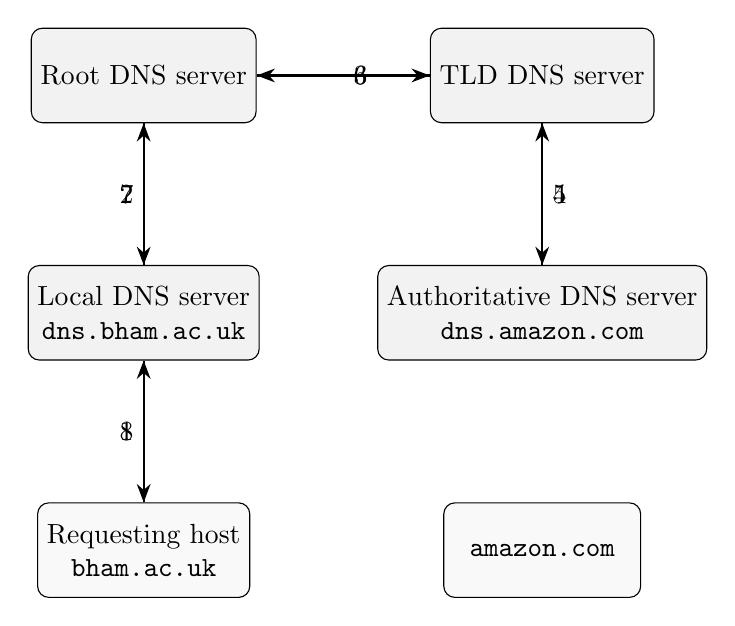
\begin{tikzpicture}[
  server/.style={draw, rounded corners, fill=gray!10, minimum width=2.8cm, minimum height=1.2cm, align=center},
  client/.style={draw, rounded corners, fill=gray!5, minimum width=2.5cm, minimum height=1.2cm, align=center},
  arrow/.style={->, thick, >=Stealth},
  node distance=1.8cm and 2.2cm
]

% Nodes
\node[client] (host) {Requesting host\\\texttt{bham.ac.uk}};
\node[server, above=of host] (local) {Local DNS server\\\texttt{dns.bham.ac.uk}};
\node[server, above=of local] (root) {Root DNS server};
\node[server, right=of root] (tld) {TLD DNS server};
\node[server, below=of tld] (auth) {Authoritative DNS server\\\texttt{dns.amazon.com}};
\node[client, below=of auth] (amazon) {\texttt{amazon.com}};

% Arrows with numbers
\draw[arrow] (host) -- node[left] {1} (local);
\draw[arrow] (local) -- node[left] {2} (root);
\draw[arrow] (root) -- node[right] {3} (tld);
\draw[arrow] (tld) -- node[right] {4} (auth);
\draw[arrow] (auth) -- node[right] {5} (tld);
\draw[arrow] (tld) -- node[right] {6} (root);
\draw[arrow] (root) -- node[left] {7} (local);
\draw[arrow] (local) -- node[left] {8} (host);

\end{tikzpicture}


To simplify the problem, assume the above data remain constant 
regardless of which server, in any country, is being contacted. Additionally, the first Root DNS server query always targets the 
geographically closest server. If this query fails, it randomly selects 
another Root DNS server, which hasn’t been tried before. What is the shortest and the longest possible time for a Local DNS server 
to resolve the query via the recursive approach as shown below?\\

\textbf{Correct Answer(s)}\\
Shortest: 210 ms\\
Longest: 310 ms\\
\textbf{Solution \& Feedback:}\\

Shortest Time: Since all Root DNS servers outside China are inaccessible, the first 
query will fail. [cite: 70, 71, 72, 73] The Local DNS will then retry until it successfully connects to one of the 
Chinese Root DNS servers:\\

\begin{itemize}
    \item Failed attempt to the nearest Root DNS server: 1 * 10 = 10 ms
    \item Successful query to a Chinese Root DNS server: 1 * 10 = 10 ms
    \item Root DNS to TLD DNS: 3 * 30 = 90 ms
    \item TLD DNS to Authoritative DNS: 2 * 50 = 100 ms
\end{itemize}

Total (shortest) = 10 + 10 + 90 + 100 = 210 ms

Longest Time: If the Local DNS server sequentially attempts all Root DNS servers, 
assuming 11 of them fail before reaching the
[cite: 72, 73] two working ones in China:

\begin{itemize}
    \item Failed attempts to the 11 inaccessible Root DNS servers (there are two root 
servers in China, so need to try 11 times before reaching to a server in China 
Mainland): 11 * 1 * 10 = 110 ms
    \item Successful attempt to one of the China Mainland DNS servers:1 * 10 = 10 ms
    \item Root DNS to TLD DNS: 3 * 30 = 90 ms
    \item TLD DNS to Authoritative DNS: 2 * 50 = 100 ms
\end{itemize}

Total (longest) = 110 + 10 + 90 + 100 = 310 ms

\subsubsection{Variation Question 8.2}

A computer virus has infected the vast majority of Root DNS servers 
globally, except for the two Root DNS servers located in China Mainland 
(due to the Great Firewall), which remain unaffected. [cite: 74, 75, 76, 77, 78, 79, 80, 81] Fortunately, the 
virus only impacts Root DNS servers, leaving Top-Level Domain (TLD) 
DNS servers and Authoritative Domain servers unharmed. [cite: 74, 75, 76, 77, 78, 79, 80, 81] Students at the 
University of Birmingham wish to resolve the DNS query for Amazon's 
website. [cite: 74, 75, 76, 77, 78, 79, 80, 81] The following data is provided:

\textbf{Round Trip Times (RTT):}

\begin{itemize}
    \item Local DNS to Root DNS: 20 ms
    \item Root DNS to TLD DNS: 40 ms
    \item TLD DNS to Authoritative DNS: 10 ms
\end{itemize}

\textbf{Query and Response Times:}

\begin{itemize}
    \item Local DNS querying the Root DNS server: 1 RTT
    \item Root DNS referring to the TLD DNS server: 2 RTT
    \item TLD DNS referring to the Authoritative DNS server: 3 RTT
\end{itemize}

To simplify the problem, assume the above data remain constant 
regardless of which server, in any country, is being contacted. [cite: 74, 75, 76, 77, 78, 79, 80, 81] Additionally, the first Root DNS server query always targets the 
geographically closest server. [cite: 74, 75, 76, 77, 78, 79, 80, 81] If this query fails, it randomly selects 
another Root DNS server, which hasn’t been tried before. [cite: 74, 75, 76, 77, 78, 79, 80, 81] What is the shortest and the longest possible time for a Local DNS server 
to resolve the query via the recursive approach as shown below?

\textbf{Correct Answer(s)}

Shortest: 150 ms

Longest: 350 ms

\textbf{Solution \& Feedback:}

Shortest Time: Since all Root DNS servers outside China are inaccessible, the first 
query will fail. [cite: 82, 83, 84] The Local DNS will then retry until it successfully connects to one of the 
Chinese Root DNS servers:

\begin{itemize}
    \item Failed attempt to the nearest Root DNS server: 1 * 20 = 20 ms
    \item Successful query to a Chinese Root DNS server: 1 * 20 = 20 ms
    \item Root DNS to TLD DNS: 2 * 40 = 80 ms
    \item TLD DNS to Authoritative DNS: 3 * 10 = 30 ms
\end{itemize}

Total (shortest) = 20 + 20 + 80 + 30 = 150 ms

Longest Time: If the Local DNS server sequentially attempts all Root DNS servers, 
assuming 11 of them fail before reaching the
[cite: 82, 83, 84] two working ones in China:

\begin{itemize}
    \item Failed attempts to the 11 inaccessible Root DNS servers (there are two root 
servers in China, so need to try 11 times before reaching to a server in China 
Mainland): 11 * 1 * 20 = 220 ms
    \item Successful attempt to one of the China Mainland DNS servers:1 * 20 = 20 ms
    \item Root DNS to TLD DNS: 2 * 40 = 80 ms
    \item TLD DNS to Authoritative DNS: 3 * 10 = 30 ms
\end{itemize}

Total (longest) = 220 + 20 + 80 + 30 = 350 ms

\subsection{Variation Question 8.3}

A computer virus has infected the vast majority of Root DNS servers 
globally, except for the two Root DNS servers located in China Mainland 
(due to the Great Firewall), which remain unaffected. [cite: 85, 86, 87, 88, 89, 90, 91, 92, 93, 94, 95] Fortunately, the 
virus only impacts Root DNS servers, leaving Top-Level Domain (TLD) 
DNS servers and Authoritative Domain servers unharmed. [cite: 85, 86, 87, 88, 89, 90, 91, 92, 93, 94, 95] Students at the 
University of Birmingham wish to resolve the DNS query for Amazon's 
website. \\
The following data is provided:\\

\textbf{Round Trip Times (RTT):}\\

\begin{itemize}
    \item Local DNS to Root DNS: 40 ms
    \item Root DNS to TLD DNS: 20 ms
    \item TLD DNS to Authoritative DNS: 25 ms
\end{itemize}

\textbf{Query and Response Times:}

\begin{itemize}
    \item Local DNS querying the Root DNS server: 5 RTT
    \item Root DNS referring to the TLD DNS server: 3 RTT
    \item TLD DNS referring to the Authoritative DNS server: 1 RTT
\end{itemize}

To simplify the problem, assume the above data remain constant 
regardless of which server, in any country, is being contacted. [cite: 85, 86, 87, 88, 89, 90, 91, 92, 93, 94, 95] Additionally, the first Root DNS server query always targets the 
geographically closest server. [cite: 85, 86, 87, 88, 89, 90, 91, 92, 93, 94, 95] If this query fails, it randomly selects 
another Root DNS server, which hasn’t been tried before. [cite: 85, 86, 87, 88, 89, 90, 91, 92, 93, 94, 95] What is the shortest and the longest possible time for a Local DNS server 
to resolve the query via the recursive approach as shown below?

\textbf{Correct Answer(s)}

Shortest: 485 ms

Longest: 2485 ms

\textbf{Solution \& Feedback:}

Shortest Time: Since all Root DNS servers outside China are inaccessible, the first 
query will fail. [cite: 93, 94, 95] The Local DNS will then retry until it successfully connects to one of the 
Chinese Root DNS servers:

\begin{itemize}
    \item Failed attempt to the nearest Root DNS server: 5 * 40 = 200 ms
    \item Successful query to a Chinese Root DNS server: 5 * 40 = 200 ms
    \item Root DNS to TLD DNS: 3 * 20 = 60 ms
    \item TLD DNS to Authoritative DNS: 1 * 25 = 25 ms
\end{itemize}

Total (shortest) = 200 + 200 + 60 + 25 = 485 ms

Longest Time: If the Local DNS server sequentially attempts all Root DNS servers, 
assuming 11 of them fail before reaching the
[cite: 93, 94, 95] two working ones in China:

\begin{itemize}
    \item Failed attempts to the 11 inaccessible Root DNS servers (there are two root 
servers in China, so need to try 11 times before reaching to a server in China 
Mainland): 11 * 5 * 40 = 2200 ms
    \item Successful attempt to one of the China Mainland DNS servers:5 * 40 = 200 ms
    \item Root DNS to TLD DNS: 3 * 20 = 60 ms
    \item TLD DNS to Authoritative DNS: 1 * 25 = 25 ms
\end{itemize}

Total (longest) = 2200 + 200 + 60 + 25 = 2485 ms

\subsection{Variation Question 9.1}

An Application Layer protocol called 2BMP (2 Byte Messaging Protocol) 
operates on source port 15119, destination port 34875 and encodes all 
its messages as two bytes. [cite: 96, 97, 98, 99, 100] Its associated Transport Layer protocol is 
UDP. [cite: 96, 97, 98, 99, 100] Following the method we discussed in the lecture, compute the 
checksum of the following 2BMP message’s associated UDP segment: 
11111111 
11110100
\textbf{Correct Answer(s) Incorrect Answers}
0011110010101110 1100001101010001
1100001101010000
0011110010101111
\textbf{Solution \& Feedback:}
Step 1. [cite: 97, 98, 99, 100] Split the UDP segment into 16-bit chunks. [cite: 97, 98, 99, 100]
Source port 
= (15119)10
= 0011101100001111
Destination port
= (34875)10
= 1000100000111011
Length 
= (8 + 2)10
= (10)10
= 0000000000001010
Message
= 1111111111110100
Step 2. [cite: 97, 98, 99, 100] Add the segments and add any carry bits back in to the LSB
Source port + destination port = X
 0011101100001111
+ 1000100000111011
= 1100001101001010
Length + message = Y
 0000000000001010
+ 1111111111111100
=10000000000000110
= 0000000000000111
X + Y
 1100001101001010
+ 0000000000000111
= 1100001101010001
Step 3. [cite: 97, 98, 99, 100] NOT the result to compute the checksum. [cite: 97, 98, 99, 100]
NOT(1100001101010001)
 = 0011110010101110
\subsection{Variation Question 9.2}

An Application Layer protocol called 16bMP (16 bit Messaging Protocol) 
operates on source port 59776, destination port 11005 and encodes all 
its messages as sixteen bits (i.e. two bytes). [cite: 100, 101] Its associated Transport 
Layer protocol is UDP. [cite: 101] Following the method we discussed in the lecture, 
compute the checksum of the following 16bMP message’s associated 
UDP segment:
00111100 
11100010
\textbf{Correct Answer(s) Incorrect Answers}
1010111010010101 1000011000111010
0101000101101001
1010111010010110
\textbf{Solution \& Feedback:}
Step 1. Split the UDP segment into 16-bit chunks. [cite: 101, 102]
Source port 
= (59776)10
= 1110100110000000
Destination port
= (11005)10
= 0010101011111101
Length 
= (8 + 2)10
= (10)10
= 0000000000001010
Message
= 0011110011100010
Step 2. Add the segments and add any carry bits back in to the LSB
Source port + destination port = X
 1110100110000000
+ 0010101011111101
=10001010001111101
= 0001010001111110
Length + message = Y
 0000000000001010
+ 0011110011100010
= 0011110011101100
X + Y
 0001010001111110
+ 0011110011101100
= 0101000101101010
Step 3. NOT the result to compute the checksum. [cite: 102, 103, 104]
NOT(0101000101101010)
 = 1010111010010101
\subsection{Variation Question 9.3}

An Application Layer protocol called 4NMP (4 nibble Messaging Protocol) 
operates on source port 32311, destination port 49555 and encodes all 
its messages as four nibbles (i.e. two bytes). Its associated Transport 
Layer protocol is UDP. Following the method we discussed in the lecture, 
compute the checksum of the following 4NMP message’s associated 
UDP segment:
10101010 
11100101\\
\textbf{Correct Answer}\\
0001010101000101 \\
\textbf{Solution \& Feedback:}\\
    
Step 1. Split the UDP segment into 16-bit chunks. 
\begin{lstlisting}
Source port 
= (32311)10
= 0111111000110111
Destination port
= (49555)10
= 1100000110010011
Length 
= (8 + 2)10
= (10)10
= 0000000000001010
Message
= 1010101011100101
\end{lstlisting}
Step 2. Add the segments and add any carry bits back in to the LSB
\begin{lstlisting}
Source port + destination port = X
 0111111000110111
+ 1100000110010011
=10011111111001010
= 0011111111001011
Length + message = Y
 0000000000001010
+ 1010101011100101
= 1010101011101111
X + Y
 0011111111001011
+ 1010101011101111
= 1110101010111010
\end{lstlisting}
Step 3. NOT the result to compute the checksum.
\begin{lstlisting}
NOT(1110101010111010)
 = 0001010101000101
\end{lstlisting}
\subsection{Variation Question 10.1}

\textbf{Question}\\
A company has 428 hosts on its network.The IP address of one host 
machine on this subnet is 167.53.11.90. Assuming the subnet has been 
designed to minimise the number of redundant addresses, what is the 
range of IP addresses in this subnet (including the network and broadcast 
addresses)?\\
\textbf{Correct Answer(s)}\\
167.53.10.0 - 167.53.11.255\\
\textbf{Solution \& Feedback:}\\
The company has 428 hosts, which means the IP addresses on its subnet will require a 
host part of minimum 9 bits (log2(428) = 8.74…).\\ 
The IP address 167.53.11.90 in binary is 10100111.00110101.00001011.01011010.
Given the host part is 9 bits, the first address owned by the subnet will be 
\underline{10100111.00110101.0000101}0.00000000 and the last address will be 
\underline{10100111.00110101.0000101}1.11111111 (the underlining delineating the subnet parts 
of the address). \\
Converting this back to denary, the range is 167.53.10.0 - 167.53.11.255. 
\subsection{Variation Question 10.2}

\textbf{Question}\\
A company has 875 hosts on its network. The IP address of one host 
machine on this subnet is 85.209.126.1. Assuming the subnet has been 
designed to minimise the number of redundant addresses, what is the 
range of IP addresses in this subnet (including the network and broadcast 
addresses)?\\
\textbf{Correct Answer(s)}\\
85.209.124.0 - 85.209.127.255\\
\textbf{Solution \& Feedback:}\\
The company has 875 hosts, which means the IP addresses on its subnet will require a 
host part of minimum 10 bits (log2(875) = 9.77…).\\
The IP address 85.209.126.1 in binary is 01010101.11010001.01111110.00000001.
Given the host part is 10 bits, the first address owned by the subnet will be 
01010101.11010001.01111100.00000000 and the last address will be 
01010101.11010001.01111111.11111111 (the underlining delineating the subnet parts 
of the address).\\
Converting this back to denary, the range is 85.209.124.0 - 85.209.127.255.

\subsection{Variation Question 10.3}

\textbf{Question}\\
A company has 1100 hosts on its network. The IP address of one host 
machine on this subnet is 1.88.5.200. Assuming the subnet has been 
designed to minimise the number of redundant addresses, what is the 
range of IP addresses in this subnet (including the network and broadcast 
addresses)?\\
\textbf{Correct Answer(s)}\\
1.88.0.0 - 1.88.7.255\\
\textbf{Solution \& Feedback:}\\
The company has 1100 hosts, which means the IP addresses on its subnet will require a 
host part of minimum 11 bits (log2(1100) = 10.103…).\\
The IP address 1.88.5.200 in binary is 00000001.01011000.00000101.11001000.
Given the host part is 11 bits, the first address owned by the subnet will be 
00000001.01011000.00000000.00000000 and the last address will be 
00000001.01011000.00000111.11111111 (the underlining delineating the subnet parts 
of the address).\\
Converting this back to denary, the range is 1.88.0.0 - 1.88.7.255.